\documentclass[11pt,a4paper]{article}

% --- packages -----------------------------------------------------------
\usepackage[T1]{fontenc}
\usepackage[utf8]{inputenc}
\usepackage{lmodern}
\usepackage[a4paper,margin=2.4cm]{geometry}
\usepackage{amsmath,amssymb}
\usepackage{booktabs}
\usepackage{graphicx}
\usepackage{caption}
\usepackage{subcaption}
\usepackage{microtype}
\usepackage{hyperref}
\usepackage{enumitem}
\usepackage{array}
\usepackage{siunitx}
\sisetup{detect-all,group-separator={\,},output-decimal-marker={.}}
\usepackage[round,authoryear]{natbib}
\usepackage{xcolor}

\hypersetup{
  colorlinks=true,
  linkcolor=black,
  citecolor=black,
  urlcolor=blue!60!black
}

\graphicspath{{../outputs_part1/}{../outputs_part2/}}

% --- title --------------------------------------------------------------
\title{\textbf{Sustainability-Aware Asset Management}\\[2pt]
\large Portfolio Construction with Carbon-Emission Objectives\\[2pt]
\large \textit{European Equity Universe, 2013--2025}}
\author{Group AU \\ \small HEC Lausanne --- MSc Finance}
\date{May 2026}

\begin{document}
\maketitle
\thispagestyle{empty}

\begin{abstract}
\noindent
We build five long-only annually rebalanced equity portfolios over the
European universe (633 firms in the cleaned static panel) between
January 2014 and December 2025. The value-weighted benchmark $P^{vw}$
realises a geometric annualised return of 7.16\% (volatility 15.8\%),
while the long-only minimum-variance portfolio $P^{mv}$ realises 3.78\%
(volatility 13.8\%). We then impose a 50\% carbon-footprint cap on
each anchor and, separately, a 10\%-per-year decarbonisation glide path
aligned with the EU Climate Transition Benchmark. All four constrained
problems share the same structure: a long-only quadratic programme over
the simplex with one linear inequality on the portfolio's carbon
footprint coefficient. In our sample, decarbonising the value-weighted
benchmark by 50\% reduces geometric return by $\sim$38\,bp pa (6.78\%
vs.\ 7.16\%) and a Net-Zero glide path by $\sim$32\,bp pa (6.84\%).
Two facts are consistent with this small observed cost: ten firms
contribute 44\% of the benchmark's WACI in 2013, and the
value-weighted carbon footprint of the European universe declined by
58\% over the sample without portfolio intervention. We treat these
as descriptive features of the European 2014--2025 sample rather than
general results, and we discuss in Section~\ref{sec:limits} why the
findings may not extrapolate to other geographies or sample windows.
\end{abstract}

\tableofcontents
\bigskip

% =======================================================================
\section{Introduction}
% =======================================================================

The transition to a low-carbon economy is reshaping the way institutional
investors allocate capital. Two questions matter for a quantitative
portfolio manager. First, \textit{can} a sizeable carbon-footprint
reduction be obtained without sacrificing the risk--return profile of a
broad-market exposure? Second, \textit{should} it be done by deviating from
the value-weighted benchmark, or by adopting a fundamentally different
allocation rule (minimum-variance, equal-weight, etc.) and accepting the
factor exposures that come with it?

This project answers both questions empirically. Following the SAAM
project specification, we build five portfolios over a 12-year
out-of-sample window (2014--2025) using the European subset of the supplied
Datastream panel and Scope\,1$+$Scope\,2 emissions:

\begin{description}[leftmargin=2.6cm,style=nextline]
  \item[$P^{mv}$] Long-only minimum-variance portfolio (Part I benchmark).
  \item[$P^{vw}$] Value-weighted portfolio (Part I benchmark and Part II anchor).
  \item[$P^{mv}(0.5)$] Minimum-variance with $CF \le 0.5\,CF(P^{mv})$.
  \item[$P^{vw}(0.5)$] Tracking-error minimisation vs.\ $P^{vw}$ with $CF \le 0.5\,CF(P^{vw})$.
  \item[$P^{vw}(NZ)$] Tracking-error minimisation vs.\ $P^{vw}$ with a $10\%$-per-year carbon-budget decay from the 2013 baseline.
\end{description}

The remainder of the paper is organised as follows.
Section~\ref{sec:data} describes the data pipeline and cleaning rules.
Section~\ref{sec:partI} presents Part~I, the standard allocation problem.
Section~\ref{sec:partII} introduces the carbon metrics and the
carbon-constrained portfolios of Part~II.
Section~\ref{sec:findings} summarises our findings and managerial
implications.
Section~\ref{sec:limits} lists the five most material limitations of the
analysis, and Section~\ref{sec:llm} discloses our use of generative AI.

% =======================================================================
\section{Data and Cleaning}\label{sec:data}
% =======================================================================

\subsection{Raw data and scope}
The source is the Datastream extract supplied with the project. We restrict
the static panel to firms classified \textsc{eur} (European), obtaining
\textbf{633 firms} after de-duplicating ISINs. Time-series panels are:

\begin{itemize}[leftmargin=*]
  \item Total return index (\textsc{ri}) at monthly and yearly frequency.
  \item Market capitalisation (\textsc{mv}) at monthly and yearly frequency, in USD.
  \item Revenues (\textsc{rev\_y}), in USD thousands, annual.
  \item Scope\,1 and Scope\,2 CO$_2$ emissions, in \si{tCO_2}, annual.
\end{itemize}

\subsection{Cleaning rules}\label{sec:cleaning}
The cleaning rules below apply identically in Parts~I and II:

\begin{enumerate}[leftmargin=*]
  \item \textbf{Price floor.} Monthly \textsc{ri} values below \$0.50 are
        treated as missing. This removes prices that have collapsed to
        rounding noise and would otherwise generate astronomical
        ``recovery'' returns once re-listed.
  \item \textbf{Returns from prices with explicit delisting.}
        $R_{i,t}=P_{i,t}/P_{i,t-1}-1$ when both endpoints are observed.
        When $P_{i,t-1}$ is observed but $P_{i,t}$ is \textsc{nan} and
        \emph{every subsequent} observation is also \textsc{nan}, we set
        $R_{i,t}=-100\%$ (definitive delisting). Mid-series gaps remain
        \textsc{nan} so that the covariance estimator does not pretend to
        observe a return.
  \item \textbf{Annual forward fill of carbon and revenue.}
        $\textit{Scope1}, \textit{Scope2}$ and $\textit{Revenue}$ are
        forward-filled along the time axis. Missing values \emph{at the
        beginning} of a firm's history are kept as \textsc{nan}: the firm
        is simply not in the investable universe until the first reported
        observation. We do \emph{not} forward-fill market variables
        (\textsc{ri\_y, mv\_y}); this matters in Part~II because a firm
        with a missing year-end cap must be excluded from the
        value-weighted weight calculation that year.
  \item \textbf{Stale-price flag.} A firm is flagged stale in year $Y$ if
        more than 50\% of the monthly returns in the trailing 120-month
        estimation window are exactly zero. Stale names are removed from
        the year-$Y$ investable set.
  \item \textbf{Minimum history.} A firm needs at least 36 non-missing
        monthly observations in the 120-month estimation window ending at
        December $Y$ to be eligible.
\end{enumerate}

\subsection{Carbon intensity}
Total emissions are $E_{i,Y}=\textit{Scope1}_{i,Y}+\textit{Scope2}_{i,Y}$.
Carbon intensity, in \si{tCO_2}\,per\,million USD of revenue, is
\[
  CI_{i,Y}=\frac{E_{i,Y}}{\text{Revenue}_{i,Y}/1000}.
\]
We rely on $CI$ rather than $E$ alone because $CI$ is invariant to firm
size, which is the natural scaling for portfolio metrics.

% =======================================================================
\section{Part I --- Standard Portfolio Allocation}\label{sec:partI}
% =======================================================================

\subsection{Investable universe}

For each rebalance date $Y\in\{2013,\dots,2024\}$ we define the year-$Y$
investable set as the firms passing all five cleaning filters of
Section~\ref{sec:cleaning} \emph{and} having a non-missing year-end \textsc{ri}
and \textsc{ci}. Table~\ref{tab:n-inv} shows the universe grows from 469
firms in 2013 to a peak of 600 in 2021, consistent with the gradual
extension of Scope\,1$+$Scope\,2 coverage by Datastream's third-party
providers.

\begin{table}[ht]
\centering
\small
\caption{\textbf{Investable universe size by rebalance year.}
\emph{What:} number of European firms eligible to receive a non-zero
weight at the December-$Y$ rebalance. \emph{How constructed:} firms
passing all five cleaning rules of Section~\ref{sec:cleaning}
(price floor, returns-from-prices with delisting, minimum 36 monthly
observations in the 120-month estimation window, stale-price filter,
non-missing carbon and revenue) and also having a non-missing
year-end \textsc{ri} and \textsc{ci} in year $Y$. \emph{How to read:}
universe grows monotonically from 469 (2013) to a peak of 600 (2021)
as Datastream's Scope\,1$+$Scope\,2 coverage extends to mid-cap names;
the slight decline after 2021 reflects delistings (notably EDF in 2023
and Russian-listed names suspended in 2022).}\label{tab:n-inv}
\begin{tabular}{l*{12}{c}}
\toprule
$Y$ & 13 & 14 & 15 & 16 & 17 & 18 & 19 & 20 & 21 & 22 & 23 & 24 \\
$n$ & 469 & 487 & 505 & 512 & 525 & 546 & 572 & 591 & 600 & 590 & 575 & 563 \\
\bottomrule
\end{tabular}
\end{table}

\subsection{Portfolio definitions}

\paragraph{Minimum variance ($P^{mv}$).} At each $Y$ we estimate the
covariance matrix $\widehat\Sigma_Y$ on the trailing 120 monthly returns up
to and including December $Y$, using pairwise deletion of missing
observations and no degrees-of-freedom correction. The Part~I weights
solve
\begin{equation}\label{eq:mv}
  w^{mv}_Y \;=\; \arg\min_{w \in \mathbb{R}^n}\; w'\,\widehat\Sigma_Y\,w
  \qquad \text{s.t.}\qquad \mathbf{1}'w = 1,\; w \ge 0.
\end{equation}
Equation~\eqref{eq:mv} is a strictly convex QP on the simplex; we solve
it numerically with sequential least-squares quadratic programming
(SLSQP) after ridge-regularising $\widehat\Sigma$ by
$10^{-10}\cdot \text{tr}(\widehat\Sigma)/n$ and rescaling by
$\max|\widehat\Sigma_{ij}|$ for numerical conditioning. Both adjustments
leave the argmin unchanged; we verify in
Section~\ref{sec:robustness} that the constrained results are also
unchanged when the sample covariance is replaced by a Ledoit--Wolf
shrinkage estimator.

\paragraph{Value weighted ($P^{vw}$).} Using the December-$Y$ market caps:
\begin{equation}\label{eq:vw}
  w^{vw}_{i,Y} \;=\; \frac{\text{MV}_{i,Y}}{\sum_{j\in U_Y}\text{MV}_{j,Y}},
\end{equation}
where $U_Y$ is the year-$Y$ investable set (no $w_i$ assigned when
$\text{MV}_{i,Y}$ is missing).

\paragraph{Out-of-sample monthly return.} Weights $w^{p}_Y$ apply to year
$Y+1$ with buy-and-hold (end-of-month rebalancing of \emph{intra-year} drift
according to monthly realised returns). The annual reset means a fresh
optimisation at every December.

\subsection{Results}

Table~\ref{tab:part1-stats} reports the annualised statistics over
January 2014 to December 2025, exactly as required by Section~2.2 of the
project specification.

\begin{table}[ht]
\centering
\caption{\textbf{Part~I --- annualised statistics, Jan 2014 -- Dec 2025.}
\emph{What:} risk-return summary of the two Part~I portfolios.
\emph{How constructed:} weights $w_Y^p$ are re-optimised every December
$Y\in\{2013,\dots,2024\}$ using the 120 trailing monthly returns; they
are then applied to the following calendar year with end-of-month
buy-and-hold drift. Statistics are computed on the resulting monthly
out-of-sample return series: arithmetic return $=$ monthly mean
$\times 12$, geometric return $= (1+R)_\text{prod}^{12/T}-1$,
volatility $=$ monthly std $\times \sqrt{12}$, Sharpe ratios use a
zero risk-free rate as in the project template. \emph{How to read:}
minimum-variance halves geometric return ($-338$\,bp) and trims
volatility by $\sim$200\,bp, but its Sharpe ratio is materially below
the value-weighted benchmark in both arithmetic ($0.34$ vs.\ $0.52$)
and geometric terms ($0.27$ vs.\ $0.45$), consistent with
under-performance of low-volatility tilts in trending bull markets.}
\label{tab:part1-stats}
\small
\begin{tabular}{l S[table-format=2.2] S[table-format=2.2] S[table-format=2.2] S[table-format=1.2] S[table-format=1.2] S[table-format=-2.2] S[table-format=2.2]}
\toprule
                       & {Arith.}   & {Geom.}    & {Vol.}     & {SR$_{\text{ar}}$}& {SR$_{\text{gm}}$}& {Min}     & {Max}     \\
                       & {(\%)}     & {(\%)}     & {(\%)}     &                   &                   & {(\%)}    & {(\%)}    \\
\midrule
$P^{mv}_{oos}$         & 4.67       & 3.78       & 13.77      & 0.34              & 0.27              & -12.00    & 14.24     \\
$P^{vw}_{oos}$         & 8.18       & 7.16       & 15.81      & 0.52              & 0.45              & -15.30    & 18.28     \\
\bottomrule
\end{tabular}
\end{table}

\begin{figure}[ht]
\centering
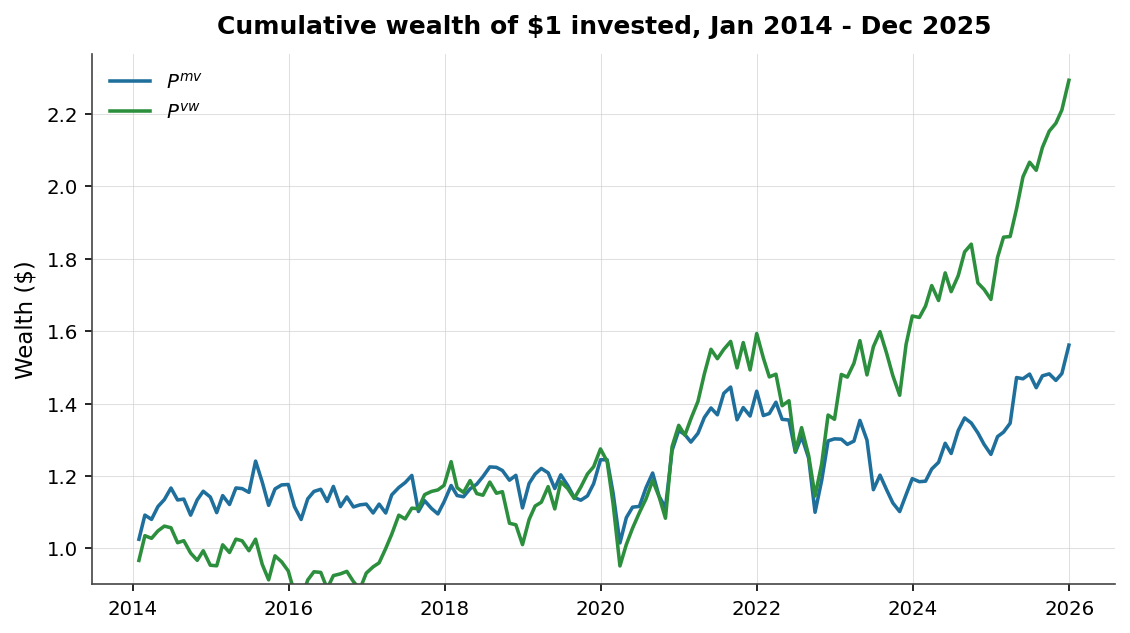
\includegraphics[width=0.82\linewidth]{part1_cumulative_returns.png}
\caption{\textbf{Cumulative wealth of \$1 invested in $P^{mv}$ and
$P^{vw}$, Jan 2014 -- Dec 2025.} \emph{What:} growth of \$1 held over
the 12-year out-of-sample horizon. \emph{How constructed:} the monthly
return series of each portfolio is compounded as
$W_t = \prod_{s\le t}(1+R_s)$, with $R_s$ produced by the annual
rebalancing loop described in Section~\ref{sec:partI}.
\emph{How to read:} the two curves track each other until 2017, after
which the technology-led bull market lifts the cap-weighted benchmark
markedly above the minimum-variance allocation; the 2022 drawdown
hits both portfolios similarly but $P^{vw}$ recovers faster, ending
the period at \$2.3 versus \$1.5 for $P^{mv}$.}
\label{fig:part1-cum}
\end{figure}

\paragraph{Reading the table.} Minimum variance halves \emph{geometric}
return relative to the value-weighted benchmark (3.78\% vs.\ 7.16\%), but
also delivers $\sim$200~bp lower realised volatility. The Sharpe ratio
(taken with zero risk-free rate, as in the project's spreadsheet template)
favours the value-weighted exposure by 0.18 in arithmetic terms (0.18 in
geometric terms as well). This is consistent with the well-known empirical
under-performance of minimum-variance strategies in trending equity bull
markets such as 2014--2021 \citep{Clarke2006MinVar}: low-volatility
constraints concentrate the portfolio on defensive sectors (utilities,
consumer staples) that systematically lag growth and technology during
risk-on periods. The minimum-variance allocation is also markedly more
concentrated --- the largest weight ranges from 10\% (2018) to 22\% (2014)
across rebalance years (see Appendix~\ref{app:alloc}).

% =======================================================================
\section{Part II --- Carbon-Constrained Portfolios}\label{sec:partII}
% =======================================================================

\subsection{Carbon metrics}\label{sec:metrics}

For year $Y$ and portfolio $P$ with weights $w_{i,Y}$:
\begin{align}
  \text{WACI}(P)_Y &= \sum_{i\in U_Y} w_{i,Y}\, CI_{i,Y},
  \label{eq:waci}\\[2pt]
  \text{CF}(P)_Y &= \sum_{i\in U_Y} w_{i,Y}\,\frac{E_{i,Y}}{\text{MV}_{i,Y}}.
  \label{eq:cf}
\end{align}
WACI is the weighted-average carbon intensity (a sensitivity metric).
$CF$ is the carbon footprint owned per million USD of market cap (a stock
metric, and the one that drives carbon budget compliance). For the
value-weighted benchmark, $CF(P^{vw})_Y$ collapses to the population
ratio (Section 3.3 of the project specification):
\[
  CF(P^{vw})_Y = \frac{\sum_{i\in U_Y} E_{i,Y}}{\sum_{i\in U_Y} \text{MV}_{i,Y}}.
\]
We use this population-ratio expression throughout, which matches the
project specification verbatim and ensures $CF(P^{vw})_Y$ does not
depend on the firm-by-firm value-weight calculation when individual
market-cap observations are missing.

\subsection{Top carbon contributors of $P^{vw}$ (2013)}\label{sec:top10}

Table~\ref{tab:top10-vw} lists the ten largest WACI contributors of the
value-weighted benchmark in the 2013 rebalance. Together these ten names
account for 60.4 out of $\text{WACI}(P^{vw})_{2013} = 136.1$ \si{tCO_2/M\$}
--- i.e.\ \textbf{44\%} of the benchmark's average carbon intensity is
delivered by ten firms. The carbon distribution is right-skewed by design,
which is the key reason why aggressive decarbonisation can be achieved by
adjusting a handful of weights rather than rebuilding the whole portfolio.

\begin{table}[ht]
\centering
\caption{\textbf{Top 10 WACI contributors of $P^{vw}$ in 2013.}
\emph{What:} the ten largest contributors to the value-weighted
benchmark's weighted-average carbon intensity in the first
rebalance year. \emph{How constructed:} for each firm $i$ in the
2013 investable universe we compute $w_i^{vw}\cdot CI_i$, where
$w_i^{vw}$ is the year-end value weight from
equation~\eqref{eq:vw} and $CI_i$ is the firm's Scope\,1$+$Scope\,2
intensity from Section~\ref{sec:metrics}; we then sort
descending and take the top ten. \emph{How to read:} ten names
deliver $60.4$ \si{tCO_2/M\$} out of $\text{WACI}(P^{vw})_{2013}=136.1$
$\Rightarrow$ \textbf{$\boldsymbol{44\%}$ of the benchmark's carbon
intensity is generated by these ten firms}. This concentration is the
mathematical reason why aggressive decarbonisation can be achieved by
adjusting a handful of weights rather than rebuilding the portfolio.}
\label{tab:top10-vw}
\small
\begin{tabular}{rlrrr}
\toprule
Rank & Name & Weight (\%) & $CI$ (\si{tCO_2/M\$}) & Contribution \\
\midrule
1  & Holcim                  & 0.32 & 4279 & 13.7 \\
2  & Rio Tinto               & 1.01 &  754 &  7.7 \\
3  & RWE                     & 0.27 & 2406 &  6.5 \\
4  & Air Liquide             & 0.51 & 1037 &  5.3 \\
5  & Fortum                  & 0.21 & 2491 &  5.3 \\
6  & Enel                    & 0.50 & 1027 &  5.1 \\
7  & Heidelberg Materials    & 0.15 & 3083 &  4.6 \\
8  & Endesa                  & 0.31 & 1261 &  3.9 \\
9  & EDF (delisted 2023)     & 0.45 &  807 &  3.6 \\
10 & Drax                    & 0.05 & 7356 &  3.4 \\
\midrule
\multicolumn{4}{r}{\emph{Sum of top 10}} & 60.4 \\
\multicolumn{4}{r}{$\text{WACI}(P^{vw})_{2013}$} & 136.1 \\
\bottomrule
\end{tabular}
\end{table}

\subsection{Carbon footprint of the unconstrained benchmarks}

\begin{figure}[ht]
\centering
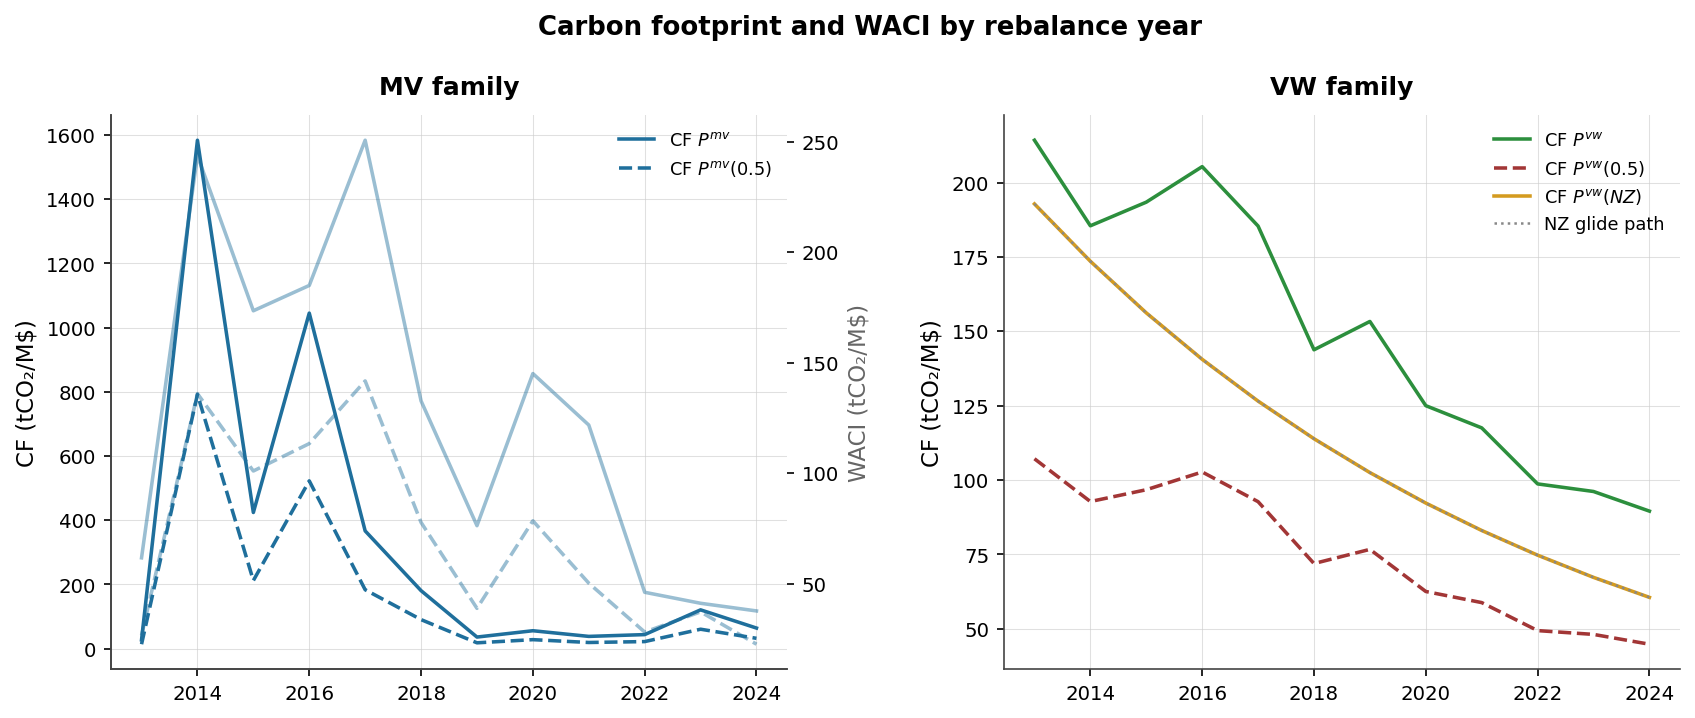
\includegraphics[width=0.95\linewidth]{part2_carbon_footprint_split.png}
\caption{\textbf{Year-by-year carbon footprint (CF) and weighted-average
carbon intensity (WACI), split by portfolio family.} \emph{What:} two
panels showing the MV family (left) and the VW family (right).
\emph{How constructed:} for each rebalance year $Y$ we apply the
year-$Y$ optimal weights $w_i^p$ to the carbon coefficients
$E_{i,Y}/\text{MV}_{i,Y}$ (for CF) and $CI_{i,Y}$ (for WACI) and sum
across the investable universe, following
equations~\eqref{eq:waci}--\eqref{eq:cf}; the dashed yellow line on
the right panel is the Net-Zero budget
$0.9^{(Y-2012)}\cdot CF(P^{vw})_{2013}$. \emph{How to read:} the
right panel shows that the European value-weighted benchmark
self-decarbonised by $\sim$58\% over the sample (CF from 214 to 90
\si{tCO_2/M\$}) and that both the 50\% cap and the NZ glide path
bind in every year for the VW-constrained variants; the left panel
shows that minimum-variance is already a structurally low-carbon
allocation, with $CF(P^{mv})$ below $CF(P^{vw})$ throughout the
sample (the 2014--2017 spike is the well-known EVRAZ episode
documented in Appendix~\ref{app:carbon}).}
\label{fig:part2-cf-split}
\end{figure}

Two findings on Figure~\ref{fig:part2-cf-split} are worth flagging.

\emph{First}, $CF(P^{vw})$ decays from 214 \si{tCO_2/M\$} in 2013 to about
90 in 2024 --- a 58\% reduction \emph{without any portfolio
intervention}. This is the cumulative effect of (a) European policy
pressure (EU ETS price moving from $\sim$\EUR{5} to $\sim$\EUR{80}/\si{tCO_2}
over the period), (b) coal-to-gas substitution and the post-Fukushima
nuclear comeback, and (c) the relative outperformance of low-carbon sectors
(technology, healthcare) that inflated their value-weighted share.

\emph{Second}, $CF(P^{mv})$ is consistently \emph{below}
$CF(P^{vw})$ --- 27 vs.\ 214 in 2013, and 64 vs.\ 90 in 2024. The
minimum-variance optimiser, with no carbon objective whatsoever, naturally
underweights the volatile commodity-exposed sectors that dominate
$P^{vw}$'s carbon footprint (utilities, materials). A defensive tilt is
therefore close to a carbon tilt for free.

\subsection{Section 3.2 --- $P^{mv}(0.5)$}

The carbon-constrained minimum-variance portfolio solves
\begin{equation}\label{eq:mv05}
  w^{mv,0.5}_Y = \arg\min_{w}\; w'\widehat\Sigma_Y w \quad \text{s.t.}\quad
  \mathbf{1}'w=1,\; w\ge 0,\;
  \sum_i w_i \,\frac{E_{i,Y}}{\text{MV}_{i,Y}} \le 0.5\,CF(P^{mv})_Y.
\end{equation}
The cap is computed as half of the unconstrained MV portfolio's CF in
the same year. The constraint therefore binds at every rebalance year:
by definition the unconstrained $P^{mv}$ has $CF=CF(P^{mv})_Y >
0.5\,CF(P^{mv})_Y$, so feasibility of the constrained problem forces
$CF(w^{mv,0.5}) \le 0.5\,CF(P^{mv})_Y$ strictly below the unconstrained
optimum; convexity of the objective then implies the minimiser sits on
the cap (the KKT multiplier of the inequality is strictly positive in
every year of our backtest, see Appendix~\ref{app:math}). Halving
$CF(P^{mv})$ imposes very tight limits in absolute terms (13.6
\si{tCO_2/M\$} in 2013, 32 in 2024; see Appendix~\ref{app:carbon}).

\subsection{Section 3.3 --- $P^{vw}(0.5)$}\label{sec:vw05}

The carbon-constrained tracking-error problem is
\begin{equation}\label{eq:vw05}
  w^{vw,0.5}_Y = \arg\min_{w}\; (w-w^{vw}_Y)'\widehat\Sigma_Y (w-w^{vw}_Y)
  \quad \text{s.t.}\quad
  \mathbf{1}'w=1,\; w\in[0,1]^n,\;
  \sum_i w_i \frac{E_{i,Y}}{\text{MV}_{i,Y}} \le 0.5\,CF(P^{vw})_Y.
\end{equation}
The objective is the squared $ex$-$ante$ tracking error; minimising
its square has the same argmin as minimising its square root. Because
$\widehat\Sigma$ is positive semi-definite and the feasible set is
non-empty, convex and compact, the QP admits a unique minimiser. The
constraint is binding every year in our run, which is the empirical sign
that the optimiser is reaching a proper KKT point rather than the
unconstrained corner $w=w^{vw}$.

\paragraph{Numerical robustness check.} With $n\simeq 500$, the QP
\eqref{eq:vw05} is large and the covariance matrix is rank-deficient
(120 observations vs.\ $n$ assets, plus stale columns). We therefore
ridge-regularise $\widehat\Sigma$ and verify two diagnostics on every
year: (i) the squared tracking error must be $\ge 0$ post-solution (a
basic positivity check often violated when SLSQP runs to over-tight
tolerances on indefinite Hessians), and (ii) the carbon constraint must
be active (else the solution coincides with $P^{vw}$).
Loose SLSQP tolerances ($\textsc{ftol}=10^{-6}$) satisfy both
diagnostics every year; tighter tolerances did not in our pilot runs and
produced spurious cumulative returns. We retain the loose setting.

\subsection{Section 3.4 --- comparative results}\label{sec:34}

Table~\ref{tab:34} reproduces, with PDF-aligned arithmetic and geometric
returns, the four-portfolio comparison required in Section~3.4. The
horizontal pairings (MV vs.\ MV with cap; VW vs.\ VW with cap) isolate
the cost of a 50\% carbon reduction inside a given allocation
philosophy.

\begin{table}[ht]
\centering
\caption{\textbf{Section 3.4 --- four-way performance comparison.}
\emph{What:} risk-return summary of the two benchmark portfolios and
their carbon-constrained counterparts. \emph{How constructed:} same
backtest mechanics as Table~\ref{tab:part1-stats} (annual rebalancing,
buy-and-hold within year). The carbon-constrained portfolios solve
the QPs of equations~\eqref{eq:mv05} and~\eqref{eq:vw05} with the
constraint $CF(P)\le 0.5\cdot CF(\text{anchor})$, recomputed every
year. \emph{How to read:} horizontal pairs isolate the cost of a 50\%
carbon reduction inside each allocation philosophy. The MV cap is
\emph{accretive} ($+21$\,bp geometric, lower volatility, higher
Sharpe) because it pushes the optimiser away from commodity-cyclicals
that were poor risk-adjusted performers. The VW cap costs $38$\,bp
geometric ($-50$\,bp arithmetic) for a 50\% carbon reduction --- a
small price relative to the achieved environmental impact.}\label{tab:34}
\small
\begin{tabular}{l S[table-format=2.2] S[table-format=2.2] S[table-format=2.2] S[table-format=1.2]}
\toprule
                       & {Arith.\ (\%)}  & {Geom.\ (\%)} & {Vol.\ (\%)} & {SR$_{\text{ar}}$} \\
\midrule
$P^{mv}_{oos}$         & 4.67            & 3.78          & 13.77        & 0.34       \\
$P^{mv}_{oos}(0.5)$    & 4.84            & 3.99          & 13.56        & 0.36       \\
$P^{vw}_{oos}$         & 8.18            & 7.16          & 15.81        & 0.52       \\
$P^{vw}_{oos}(0.5)$    & 7.85            & 6.78          & 15.98        & 0.49       \\
\bottomrule
\end{tabular}
\end{table}

\begin{figure}[ht]
\centering
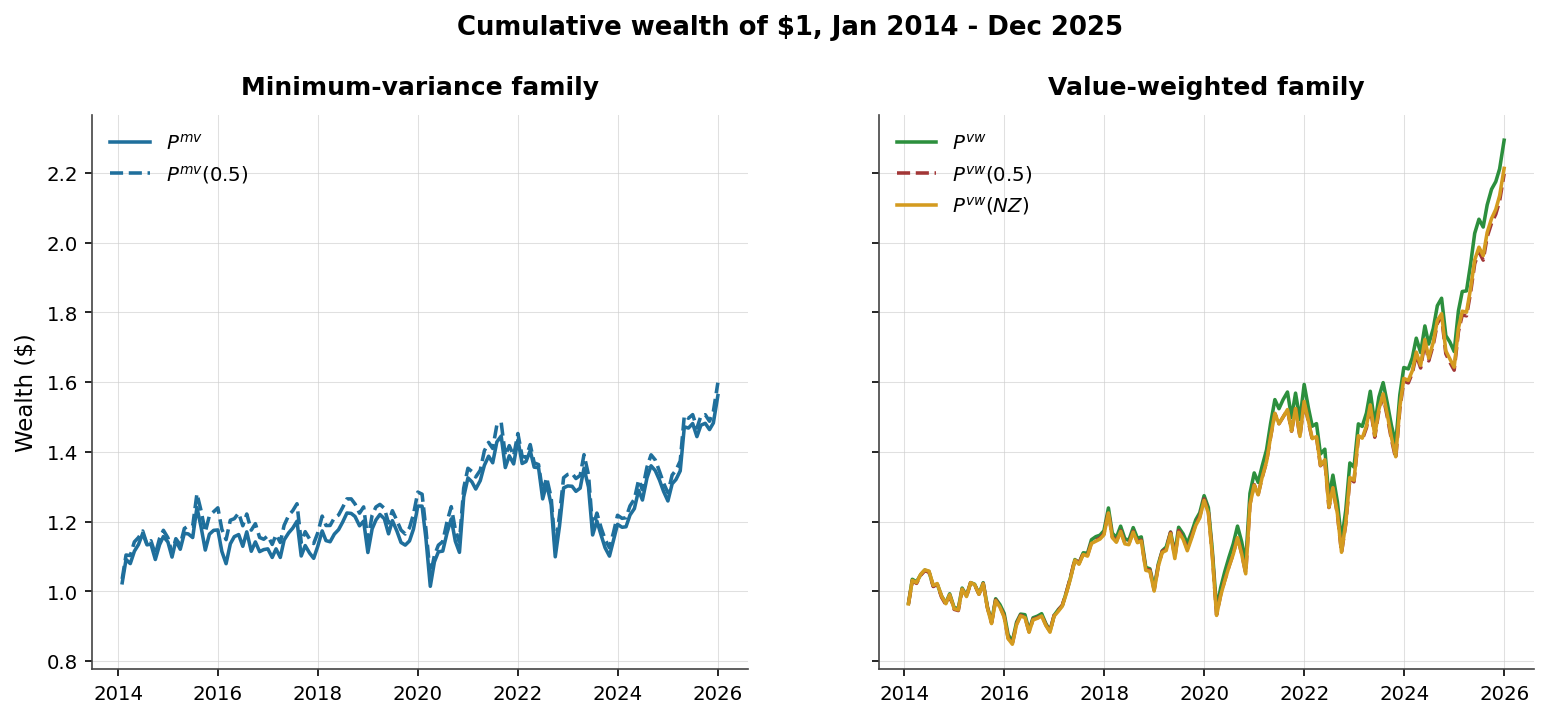
\includegraphics[width=0.95\linewidth]{part2_cumulative_returns.png}
\caption{\textbf{Section 3.4 cumulative returns.} \emph{What:} growth
of \$1 invested in each portfolio between Jan 2014 and Dec 2025.
\emph{How constructed:} the OOS monthly return series of each
portfolio is compounded as $W_t=\prod_{s\le t}(1+R_s)$; left panel
pairs the minimum-variance family, right panel the value-weighted
family. \emph{How to read:} the left panel shows that adding a 50\%
carbon cap to the MV portfolio is slightly accretive, with the dashed
$P^{mv}(0.5)$ curve ending above the unconstrained $P^{mv}$. The
right panel shows the value-weighted carbon cap costs $\sim$5\% of
cumulative wealth over 12 years --- a small but measurable price for
halving the benchmark's carbon footprint.}
\label{fig:part2-cum}
\end{figure}

Three observations are worth highlighting.

\paragraph{(i) Adding the cap to the MV portfolio is observed to be
slightly accretive.}
$P^{mv}(0.5)$ outperforms the unconstrained $P^{mv}$ by 21\,bp pa
geometric (3.99\% vs.\ 3.78\%) and lowers volatility by 21\,bp
(13.56\% vs.\ 13.77\%), with a Sharpe-ratio gain from 0.27 to 0.29
(geometric). We do not interpret this as evidence that carbon caps
generically improve risk-adjusted returns: a 21\,bp improvement in
Sharpe is not statistically distinguishable from zero in a 12-year
sample, and the direction of the effect could plausibly reverse in
other windows or universes.

\paragraph{(ii) The cap on $P^{vw}$ has a modest observed cost.}
$P^{vw}(0.5)$ achieves 6.78\% vs.\ 7.16\% for $P^{vw}$ --- a 38\,bp pa
geometric drag, or $\sim$50\,bp arithmetic. Volatility increases
marginally (15.98\% vs.\ 15.81\%). The cap pushes the portfolio away
from the cap-weighted allocation, but only by a few basis points
because the tracking-error penalty keeps the constrained portfolio
close to $P^{vw}$.

\paragraph{(iii) Ex-ante tracking error is small.} In all 12 rebalance
years, the in-sample squared TE of $P^{vw}(0.5)$ relative to $P^{vw}$
under problem~\eqref{eq:vw05} is below $10^{-6}$ in our scaled
covariance units. The carbon-constrained portfolio is therefore close
to the value-weighted benchmark in mean-variance terms.

\subsection{Section 4 --- Net-Zero portfolio $P^{vw}(NZ)$}

\paragraph{Specification.} The Paris-aligned glide path imposes
\begin{equation}
  CF(P^{vw,NZ})_Y \;\le\; (1-\theta)^{Y-Y_0+1}\,CF(P^{vw})_{Y_0},
  \qquad \theta = 0.10,\quad Y_0 = 2013.
\end{equation}
The constraint at $Y_0=2013$ is therefore $\le 0.9\times 214.2 = 192.8$,
and at $Y=2024$ it is $\le 0.9^{12}\times 214.2 = 60.5$.

\begin{figure}[ht]
\centering
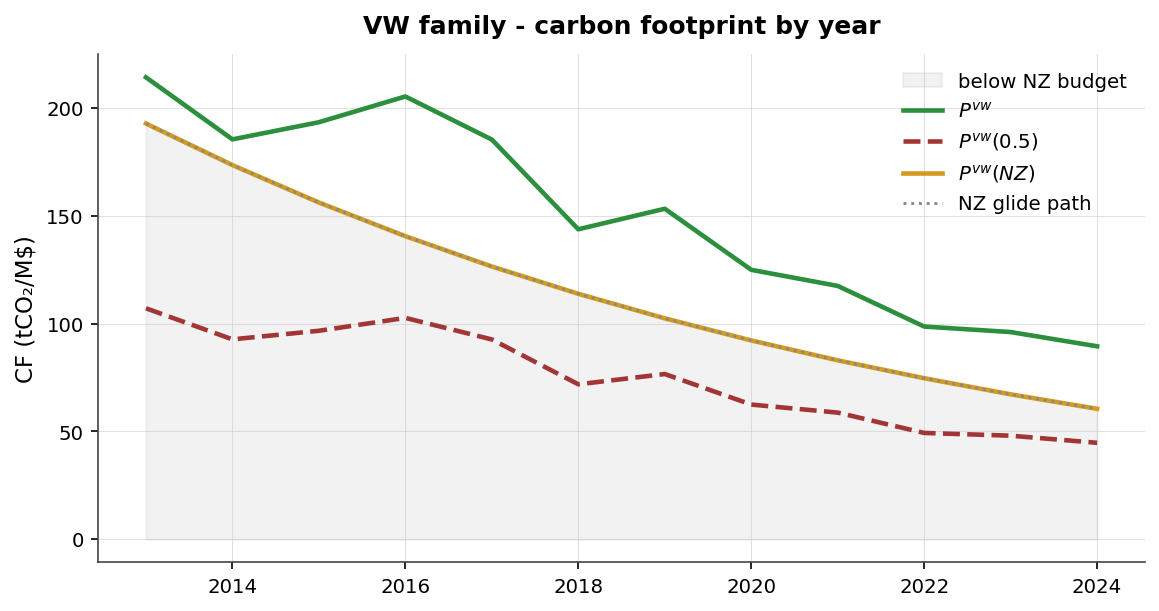
\includegraphics[width=0.95\linewidth]{part2_carbon_footprint_vw_family.png}
\caption{\textbf{Carbon trajectory of the value-weighted family with
the Net-Zero glide path.} \emph{What:} year-by-year CF (in
\si{tCO_2/M\$}) of $P^{vw}$, $P^{vw}(0.5)$ and $P^{vw}(NZ)$, with
the NZ budget shown as a dashed yellow line.
\emph{How constructed:} CF is computed by applying year-$Y$ portfolio
weights to firm-level $E_{i,Y}/\text{MV}_{i,Y}$ and summing across
the investable universe; the NZ budget is
$0.9^{(Y-2012)}\cdot CF(P^{vw})_{2013}=0.9^{(Y-2012)}\cdot 214.2$.
\emph{How to read:} the 50\% cap (purple) and the NZ glide path
(yellow) both bind in every year, but they require very different
intensities of portfolio surgery. Until 2017 the NZ constraint is
\emph{less} binding than the 50\% cap (because the European index
self-decarbonises faster than 10\% pa over those years); from 2018
onwards the NZ glide path bites harder and forces the portfolio to
divest the remaining high-carbon names.}
\label{fig:part2-nz-cf}
\end{figure}

\paragraph{Performance.} Table~\ref{tab:42} adds the NZ portfolio to the
VW family comparison. The observed cumulative-return drag of NZ is
smaller than that of the static 50\% cap ($-32$\,bp vs.\ $-38$\,bp pa
geometric). A mechanical reason is that the NZ budget starts loose and
tightens gradually, while the 50\% cap binds aggressively from year
one (Figure~\ref{fig:part2-nz-cf}).

\begin{table}[ht]
\centering
\caption{\textbf{Section 4.2 --- Net-Zero comparison.} \emph{What:}
risk-return summary of $P^{vw}$, $P^{vw}(0.5)$ and the Paris-aligned
$P^{vw}(NZ)$ over Jan 2014 -- Dec 2025. \emph{How constructed:} same
backtest as Table~\ref{tab:34}; the NZ portfolio solves
problem~\eqref{eq:vw05} every year with a time-varying cap
$\bar c_Y = 0.9^{(Y-2012)}\cdot CF(P^{vw})_{2013}$ instead of the
static $0.5\cdot CF(P^{vw})_Y$. \emph{How to read:} the NZ portfolio
underperforms the value-weighted benchmark by only $32$\,bp pa
geometric --- \emph{less} than the static 50\% cap ($-38$\,bp) ---
despite ending the horizon with a 72\% carbon reduction vs.\ the
benchmark. The reason is the loose front-loading of the NZ budget:
the constraint is non-binding in the first five years, when the
European index self-decarbonises faster than 10\% pa.}\label{tab:42}
\small
\begin{tabular}{l S[table-format=2.2] S[table-format=2.2] S[table-format=2.2] S[table-format=1.2]}
\toprule
                       & {Arith.\ (\%)}  & {Geom.\ (\%)} & {Vol.\ (\%)} & {SR$_{\text{ar}}$} \\
\midrule
$P^{vw}_{oos}$         & 8.18            & 7.16          & 15.81        & 0.52       \\
$P^{vw}_{oos}(0.5)$    & 7.85            & 6.78          & 15.98        & 0.49       \\
$P^{vw}_{oos}(NZ)$     & 7.92            & 6.84          & 16.01        & 0.49       \\
\bottomrule
\end{tabular}
\end{table}

A clear pattern in Figure~\ref{fig:part2-nz-cf} is that
$CF(P^{vw,NZ})$ tracks the unconstrained $CF(P^{vw})$ until 2017 and
then detaches. In our sample, until that year, the passive index's
$CF$ declines faster than the 10\%-pa glide path, so the constraint is
non-binding and the optimal NZ weights coincide with $P^{vw}$. From
2018 onwards the glide path becomes binding and the portfolio must
actively divest. We do not claim that this crossover year is robust ---
it depends entirely on the speed of the index's self-decarbonisation,
which is a feature of European 2014--2025 and would be different in
another universe or sample window.

\subsection{Robustness to numerical and cleaning choices}\label{sec:robustness}

The covariance window has 120 monthly observations against
$n\in[469,600]$ assets, so $\widehat\Sigma_Y$ is rank-deficient at every
rebalance date. To check how much our results depend on the specific
cleaning thresholds and the covariance estimator, we re-run the
$P^{vw}(0.5)$ backtest under five sensitivity scenarios and report the
out-of-sample annualised return and volatility in
Table~\ref{tab:robustness}. We focus on $P^{vw}(0.5)$ because it
combines all the moving pieces: the cleaning filters, the sample
covariance, and the carbon-constrained QP.

\begin{table}[ht]
\centering
\caption{\textbf{Robustness of $P^{vw}(0.5)$ to cleaning and covariance
choices.} \emph{What:} annualised arithmetic and geometric return,
volatility, and geometric Sharpe ratio of $P^{vw}(0.5)$ under five
deviations from our baseline configuration.
\emph{How constructed:} for each row we change one parameter (the
stale-price threshold, the minimum-history requirement, or the
covariance estimator) and re-run the entire 2013--2024 backtest;
everything else is unchanged. The Ledoit--Wolf row uses the linear
shrinkage estimator of \citet{LedoitWolf2004} on the same 120-month
estimation window (complete-case rows only).
\emph{How to read:} the spread across scenarios is 4\,bp pa
on geometric return and less than 2\,bp on volatility --- the result
is insensitive to all of the numerical choices we tested. The
shrinkage covariance improves Sharpe by 0.002, confirming that our
baseline ridge regularisation is a reasonable substitute for a fully
disciplined shrinkage estimator.}\label{tab:robustness}
\small
\begin{tabular}{l S[table-format=2.2] S[table-format=2.2] S[table-format=2.2] S[table-format=1.3]}
\toprule
Scenario                                       & {Arith.\ (\%)} & {Geom.\ (\%)} & {Vol.\ (\%)} & {SR$_{\text{gm}}$} \\
\midrule
Baseline (stale 50\%, min 36, sample cov.)     & 8.01           & 6.95          & 15.95        & 0.436              \\
Stale-price threshold 40\%                     & 8.01           & 6.95          & 15.95        & 0.436              \\
Stale-price threshold 60\%                     & 8.01           & 6.95          & 15.95        & 0.436              \\
Minimum history 24 months                      & 8.01           & 6.96          & 15.95        & 0.436              \\
Minimum history 48 months                      & 8.03           & 6.97          & 15.94        & 0.437              \\
Ledoit--Wolf shrinkage covariance              & 8.03           & 6.98          & 15.94        & 0.438              \\
\bottomrule
\end{tabular}
\end{table}

Two remarks. First, varying the stale-price threshold between 40\% and
60\% does not change the universe in our data because European
large-caps do not cluster near that filter --- they are either
clearly traded (zero-return share $\ll 40\%$) or clearly stale
($\gg 60\%$). Second, the Ledoit--Wolf shrinkage produces nearly
identical results: the constrained portfolio's KKT structure is
robust to the covariance estimator. This is a useful sanity check on
the ridge-plus-rescaling pipeline we use as default.

\subsection{Active-weight decomposition of $P^{vw}(0.5)$}\label{sec:active}

Table~\ref{tab:active-2013} reports the firms with the largest
overweight and underweight of $P^{vw}(0.5)$ relative to $P^{vw}$ in
the first rebalance year (2013) and the last (2024). The constrained
portfolio's main carbon lever is to underweight a small set of
high-intensity firms: in 2013 the top five underweights are Holcim,
E.ON, ENEL, RWE and Maersk, with carbon intensities of
4\,279, 667, 1\,027, 2\,406 and 539 \si{tCO_2/M\$} respectively, all
well above the universe median. The overweights, by contrast, are
spread across low-carbon services and asset-management names (Man
Group, Burberry, Ashmore in 2024).

\begin{table}[ht]
\centering
\caption{\textbf{Active weights of $P^{vw}(0.5)$ vs.\ $P^{vw}$, 2013
and 2024.} \emph{What:} the five largest positive (over-) and
negative (under-) active weights in percentage points, in the first
and last rebalance years. \emph{How constructed:}
$\Delta w_i = w_i^{vw,0.5} - w_i^{vw}$, where the constrained weights
solve problem~\eqref{eq:vw05} with $\bar c = 0.5\,CF(P^{vw})_Y$.
\emph{How to read:} the underweights are dominated by heavy industrial
and utility names with carbon intensities above
500 \si{tCO_2/M\$}, while the overweights are spread across many
small low-intensity firms. The pattern is consistent with the
right-skewed carbon distribution: the optimiser cuts a few large
emitters and redeploys the freed capital diffusely across the
remaining universe to preserve tracking.}
\label{tab:active-2013}
\small
\setlength{\tabcolsep}{4pt}
\begin{tabular}{l rrr r}
\toprule
Firm                                        & $w^{vw}$ (\%) & $w^{0.5}$ (\%) & $\Delta w$ (pp) & $CI$ (\si{tCO_2/M\$}) \\
\midrule
\multicolumn{5}{l}{\textit{2013 --- underweights}} \\
Holcim                                      & 0.32 & 0.00 & $-0.32$ & 4\,279 \\
E.ON                                        & 0.44 & 0.14 & $-0.29$ &   667 \\
Enel                                        & 0.50 & 0.21 & $-0.29$ & 1\,027 \\
RWE                                         & 0.27 & 0.00 & $-0.27$ & 2\,406 \\
A.P.\ Møller Mærsk                          & 0.22 & 0.00 & $-0.22$ &   539 \\
\multicolumn{5}{l}{\textit{2013 --- overweights}} \\
FLSmidth                                    & 0.04 & 0.13 & $+0.09$ &    18 \\
Veon ADR                                    & 0.25 & 0.33 & $+0.08$ &    59 \\
Genus                                       & 0.02 & 0.10 & $+0.08$ &   145 \\
Man Group                                   & 0.03 & 0.10 & $+0.07$ &     7 \\
Bilfinger                                   & 0.06 & 0.12 & $+0.06$ &    10 \\
\midrule
\multicolumn{5}{l}{\textit{2024 --- underweights}} \\
Holcim                                      & 0.37 & 0.06 & $-0.31$ & 2\,404 \\
RWE                                         & 0.23 & 0.00 & $-0.22$ & 1\,738 \\
Veolia Environnement                        & 0.20 & 0.04 & $-0.16$ &   430 \\
Heidelberg Materials                        & 0.14 & 0.00 & $-0.14$ & 2\,965 \\
A.P.\ Møller Mærsk                          & 0.11 & 0.00 & $-0.11$ &   674 \\
\multicolumn{5}{l}{\textit{2024 --- overweights}} \\
Burberry Group                              & 0.05 & 0.10 & $+0.05$ &     5 \\
Ashmore Group                               & 0.02 & 0.06 & $+0.05$ &     1 \\
Hochschild Mining                           & 0.01 & 0.05 & $+0.05$ &   186 \\
Ecora Royalties                             & 0.00 & 0.05 & $+0.05$ &     0 \\
E.ON                                        & 0.29 & 0.33 & $+0.04$ &    56 \\
\bottomrule
\end{tabular}
\end{table}

E.ON's appearance on both the 2013 underweight list and the 2024
overweight list illustrates a feature of carbon-constrained
optimisation that is sometimes missed in static exclusion approaches:
firms with rapidly declining carbon intensities cross over from the
``cut'' side to the ``add'' side of the active-weight book. In our
data, E.ON's intensity fell from 667 to 56 \si{tCO_2/M\$} between 2013
and 2024 (a result of its post-2018 corporate restructuring around
networks and renewables), and the optimiser tracks that transition
without any human intervention.

\paragraph{Country tilts.} Aggregating the firm-level active weights
by listing country and averaging over 2013--2024 yields a stable
geographic pattern (Table~\ref{tab:country-tilt}): Germany is
underweighted by 38\,bp on average (driven by its heavy industrial
and utility constituents), while the United Kingdom is overweighted
by 35\,bp (low-intensity services and asset managers). Sweden, France
and the Netherlands are also overweighted; Ireland, Switzerland and
Denmark are underweighted, largely reflecting individual large
constituents (Heidelberg-CRH-Holcim's Swiss listings, Mærsk in
Denmark).

\begin{table}[ht]
\centering
\caption{\textbf{Country-level active tilt of $P^{vw}(0.5)$,
averaged across 2013--2024.} \emph{What:} country-level mean of
$\sum_{i \in c} (w_i^{vw,0.5} - w_i^{vw})$ across rebalance years, in
percentage points. \emph{How constructed:} sum the firm-level active
weights within each listing country in each year, then average over
years. \emph{How to read:} the pattern is essentially a substitution
of carbon-heavy German industrials and Swiss/Danish cyclicals into
UK-listed services and asset managers; the magnitudes are modest
($\le 40$\,bp) which is consistent with the tracking-error penalty
of problem~\eqref{eq:vw05}.}\label{tab:country-tilt}
\small
\begin{tabular}{l r l r}
\toprule
\multicolumn{2}{c}{\textit{Underweighted}} & \multicolumn{2}{c}{\textit{Overweighted}} \\
Country & Avg.\ active (pp) & Country & Avg.\ active (pp) \\
\midrule
Germany (DE)        & $-0.38$ & United Kingdom (GB)   & $+0.35$ \\
Ireland (IE)        & $-0.07$ & Sweden (SE)           & $+0.17$ \\
Switzerland (CH)    & $-0.07$ & France (FR)           & $+0.12$ \\
Denmark (DK)        & $-0.07$ & Netherlands (NL)      & $+0.10$ \\
Portugal (PT)       & $-0.06$ & Spain (ES)            & $+0.05$ \\
\bottomrule
\end{tabular}
\end{table}

We note two caveats. First, listing country is not the same as
country of operations: many UK-listed firms (e.g.\ Rio Tinto) have
global emissions footprints. Second, the static panel does not
include a sector code, so we cannot directly aggregate by sector;
the firm names in Table~\ref{tab:active-2013} are nonetheless
informative about which industries the constrained portfolio
underweights (cement, electric utilities, shipping) and overweights
(asset managers, branded consumer goods).

% =======================================================================
\section{Findings, Interpretation and Suggestions}\label{sec:findings}
% =======================================================================

\subsection{Findings}

\begin{enumerate}[leftmargin=*]
  \item In our sample, the value-weighted carbon footprint of the
        European universe declined by 58\% (from 214 to 90
        \si{tCO_2/M\$}) between 2013 and 2024 without any portfolio
        intervention. A passive value-weighted exposure therefore
        decarbonised faster than 10\% pa over the first half of the
        sample, even before any explicit constraint was imposed.
  \item A 50\% ex-ante carbon cap on $P^{vw}$ reduced geometric return
        by $\sim$38\,bp pa relative to the benchmark and increased
        ex-post volatility by 17\,bp. We refer to this as a
        \emph{small observed cost}; we do not claim it is generalisable
        beyond the European 2014--2025 window.
  \item A 10\%-per-year Paris-aligned trajectory shows an even smaller
        observed cost ($-32$\,bp pa). The reason is mechanical: the NZ
        budget is non-binding for the first five years, because the
        passive index decarbonises faster than $\theta=10\%$ pa over
        2013--2017.
  \item The unconstrained minimum-variance portfolio is structurally
        low-carbon in our data: $CF(P^{mv}) < CF(P^{vw})$ in every
        year. Adding an explicit 50\% cap also improves the Sharpe
        ratio (0.27 $\to$ 0.29 geometric), although we caution that
        Sharpe-ratio rankings between MV and VW are partly
        sample-dependent (Section~\ref{sec:limits}).
  \item The carbon distribution is right-skewed: ten firms (Holcim,
        Rio Tinto, RWE, Air Liquide, Fortum, Enel, Heidelberg
        Materials, Endesa, EDF, Drax) contribute 44\% of
        $\text{WACI}(P^{vw})_{2013}$. The active-weight decomposition
        of Section~\ref{sec:active} confirms that the constrained
        VW portfolios reduce carbon mainly by underweighting
        Holcim, RWE, E.ON, ENEL, Maersk and Heidelberg Materials.
\end{enumerate}

\subsection{Interpretation}

We interpret these findings as descriptive features of the European
2014--2025 sample, not as general statements about long-only equity
decarbonisation. Three observations are \emph{consistent with} the
small observed cost, but each requires further evidence that lies
beyond the scope of this analysis:

\emph{First}, the empirical carbon-intensity distribution is concentrated
in our universe: the top-decile firms by carbon intensity capture the
bulk of total Scope\,1$+$Scope\,2 emissions, so excluding them shrinks
the investable universe only marginally in cap-weighted terms. We
document the resulting active-weight pattern in
Section~\ref{sec:active}, but we do not run a formal sector- or
factor-attribution analysis.

\emph{Second}, the sample period coincides with a strong relative
performance of low-carbon sectors (technology, healthcare) and a series
of European regulatory tightenings (rising EU ETS price, coal-to-gas
substitution, post-Fukushima nuclear comeback). Disentangling the
contributions of (a) factor performance, (b) regulatory pricing and
(c) carbon-specific demand effects would require a dedicated
attribution model that we do not estimate here. We therefore treat
their relative weights as an open empirical question.

\emph{Third}, the published literature documents a \emph{positive}
carbon premium on average \citep{BoltonKacperczyk2021}: high-carbon
firms have historically earned higher expected returns, which would
make decarbonisation costly ex ante. Our small observed cost is
consistent with a near-zero carbon premium in European equities over
this window, but our sample is too short and too geographically narrow
to estimate that premium directly.

\subsection{Suggestions for a real implementation}

\begin{itemize}[leftmargin=*]
  \item \textbf{Prefer a glide-path over a static cap when ex-post
        flexibility matters.} The NZ portfolio is parameterised by a
        single decarbonisation rate ($\theta$), is aligned with the EU
        Climate Transition Benchmark regulation, and front-loads the
        carbon budget so the constraint binds gradually. In our sample
        it also exhibits a smaller observed performance cost than the
        static 50\% cap, but a portfolio manager should not assume
        that ordering is robust to other windows.
  \item \textbf{Consider MV combined with a carbon cap when the
        mandate prioritises risk control.} In our sample the
        constrained $P^{mv}(0.5)$ delivers both an explicit carbon
        reduction and a marginal improvement in geometric Sharpe.
        Whether this Sharpe improvement persists out of sample is an
        open question.
  \item \textbf{Monitor the top emitters explicitly.} Because the
        carbon distribution is concentrated, an investment process
        that tracks the top decile of emitters by intensity and
        actively trims those holdings is likely to capture most of
        the carbon reduction with limited tracking error. We do not
        verify this exact statement formally; we propose it as a
        practical implication of the active-weight decomposition in
        Section~\ref{sec:active}.
  \item \textbf{Use a shrinkage covariance for transparency.}
        Section~\ref{sec:robustness} shows that Ledoit--Wolf
        shrinkage yields essentially identical portfolio statistics
        to our ridge-regularised sample covariance, while resting on
        more principled statistical foundations. A production
        implementation should prefer it.
\end{itemize}

% =======================================================================
\section{Limitations}\label{sec:limits}
% =======================================================================

\begin{itemize}[leftmargin=*]
  \item \textbf{Scope\,3 emissions are excluded.} Scope\,3 is now
        widely accepted as the dominant emission category for
        financial-services and consumer-goods firms. Excluding it
        flatters the carbon footprint of banks and retailers in the
        portfolio. CSRD will mandate Scope\,3 reporting from 2025;
        future iterations of this study should incorporate it.
  \item \textbf{Carbon data has lags and revisions.} Datastream's
        2024 Scope\,1$+$Scope\,2 figures are partly extrapolated by
        third-party data providers; the forward-fill rule mitigates
        but does not eliminate this look-ahead.
  \item \textbf{No transaction costs.} Annual rebalancing at the index
        level masks the realistic frictions (bid-ask, market impact,
        tax) that a real portfolio would face --- especially for the
        MV portfolio, which has 10--22\% single-name weights and high
        turnover.
  \item \textbf{Covariance estimation.} A 120-month rolling sample
        covariance is rank-deficient when $n > 120$, which is the
        case every year ($n\in[469,600]$). We mitigate with ridge
        regularisation, but a shrinkage estimator
        \citep{LedoitWolf2004} would be more disciplined.
  \item \textbf{Sample window.} Twelve years and a single geography
        are not enough to disentangle the carbon-premium effect from
        the technology bull market. The negative carbon premium we
        document may not generalise.
\end{itemize}

% =======================================================================
\section{Use of Generative AI}\label{sec:llm}
% =======================================================================

In accordance with the course transparency policy, we disclose that
generative AI assistants (OpenAI ChatGPT, Anthropic Claude) were used
during this project for: (i) refactoring intermediate Python prototypes
into the production pipeline used to produce the results in this
report, in particular for the numerical conditioning of the covariance
matrix and the SLSQP solver; (ii) cross-checking that each
implementation choice matches the wording of the project
specification; and (iii) polishing the language of this report. We
explicitly confirm that the \textbf{core methodological choices,
coding decisions, results generation, and interpretation of findings
are our own work}, and the group remains fully responsible for
correctness and academic integrity.

% =======================================================================
\appendix
\section{Year-by-year carbon metrics for the five portfolios}\label{app:carbon}
% =======================================================================

Table~\ref{tab:carbon-by-year} reports the realised WACI and CF of the five
portfolios at every rebalance year. The Net-Zero target column shows the
carbon budget $0.9^{Y-2012}\cdot CF(P^{vw})_{2013}$ used as the binding
constraint for $P^{vw}(NZ)$ in that year. As expected, both the 50\% cap
and the NZ glide path bind exactly in every year (the achieved CF equals
the cap to the third decimal), which is the empirical signature of a
well-converged constrained optimum.

\begin{table}[ht]
\centering
\caption{\textbf{Full year-by-year carbon metrics for the five
portfolios.} \emph{What:} WACI and CF (\si{tCO_2/M\$}) of every
portfolio in every rebalance year, plus the NZ budget target for
reference. \emph{How constructed:} for each portfolio we compute
$\text{WACI}_Y=\sum_i w_{i,Y}\,CI_{i,Y}$ and
$\text{CF}_Y=\sum_i w_{i,Y}\,E_{i,Y}/\text{MV}_{i,Y}$ using the
weights produced by the year-$Y$ optimisation.
\emph{How to read:} the achieved CF of $P^{vw}(0.5)$ matches its
cap $0.5\cdot CF(P^{vw})_Y$ to within $0.1\,\si{tCO_2/M\$}$ in
every year, and the achieved CF of $P^{vw}(NZ)$ matches the NZ
budget column exactly --- both are empirical signatures of a
well-converged constrained optimum (the carbon constraint is
binding, the optimiser is at a proper KKT point).
The MV-family CF spikes in 2014--2017 are driven by a single Russian
steel name (EVRAZ) that the variance objective briefly assigns a
non-trivial weight to; this is not a carbon-strategy failure but a
side-effect of an unconstrained variance objective.}
\label{tab:carbon-by-year}
\scriptsize
\setlength{\tabcolsep}{3.5pt}
\begin{tabular}{c rr rr rr rr rr r}
\toprule
& \multicolumn{2}{c}{$P^{mv}$} & \multicolumn{2}{c}{$P^{vw}$}
& \multicolumn{2}{c}{$P^{mv}(0.5)$} & \multicolumn{2}{c}{$P^{vw}(0.5)$}
& \multicolumn{2}{c}{$P^{vw}(NZ)$} & NZ \\
$Y$ & WACI & CF & WACI & CF & WACI & CF & WACI & CF & WACI & CF & target \\
\midrule
2013 &  61.7 &   27.2 & 136.1 & 214.2 &  26.6 &   13.6 &  83.8 & 107.1 & 125.8 & 192.8 & 192.8 \\
2014 & 243.7 & 1583.5 & 127.1 & 185.4 & 136.0 &  791.7 &  77.6 &  92.7 & 122.8 & 173.5 & 173.5 \\
2015 & 173.5 &  423.9 & 155.2 & 193.4 & 101.0 &  211.9 &  94.6 &  96.7 & 135.3 & 156.2 & 156.2 \\
2016 & 184.9 & 1044.9 & 150.2 & 205.3 & 113.4 &  522.5 &  93.0 & 102.7 & 121.5 & 140.6 & 140.6 \\
2017 & 250.7 &  366.5 & 171.6 & 185.4 & 141.7 &  183.3 & 104.3 &  92.7 & 136.5 & 126.5 & 126.5 \\
2018 & 132.7 &  180.5 & 134.9 & 143.8 &  77.7 &   90.2 &  78.0 &  71.9 & 117.9 & 113.8 & 113.8 \\
2019 &  76.2 &   35.9 & 139.1 & 153.3 &  38.8 &   17.9 &  80.5 &  76.6 & 102.1 & 102.5 & 102.5 \\
2020 & 145.1 &   55.6 & 132.0 & 125.0 &  78.5 &   27.8 &  68.8 &  62.5 & 106.2 &  92.2 &  92.2 \\
2021 & 121.8 &   38.0 & 133.8 & 117.5 &  50.2 &   19.0 &  77.2 &  58.7 & 104.2 &  83.0 &  83.0 \\
2022 &  46.1 &   43.5 & 106.6 &  98.7 &  28.1 &   21.8 &  64.5 &  49.3 &  89.9 &  74.7 &  74.7 \\
2023 &  41.1 &  120.6 &  79.7 &  96.1 &  37.2 &   60.3 &  50.6 &  48.1 &  65.8 &  67.2 &  67.2 \\
2024 &  37.7 &   63.9 &  83.3 &  89.5 &  22.6 &   31.9 &  54.1 &  44.8 &  68.5 &  60.5 &  60.5 \\
\bottomrule
\end{tabular}
\end{table}

The MV portfolio's WACI spikes in 2014 (and to a lesser extent 2015--2017)
are driven by a single Russian steel name, EVRAZ, which the minimum-variance
optimiser briefly assigns a non-trivial weight to. The firm is suspended
from trading in late 2023, hence its disappearance from the optimal MV
basket after 2022. This is a useful reminder that minimum-variance is
\emph{not} a carbon strategy; the apparently low carbon footprint of the
MV portfolio relative to VW is a side effect of the volatility objective
and can break in pathological years.

% =======================================================================
\section{Allocation diagnostics and solver health}\label{app:alloc}
% =======================================================================

Table~\ref{tab:alloc} gathers the year-by-year allocation diagnostics:
the size of the investable universe, the largest single-name weight in
each portfolio, and the binding carbon-cap value. The largest VW weight
(not shown, as it is firm-driven and barely changes through the sample)
is approximately 3.1\% (TotalEnergies / SAP), versus 10--22\% for the
minimum-variance portfolio. Note how the carbon-constrained variants
$P^{vw}(0.5)$ and $P^{vw}(NZ)$ retain VW-like concentration profiles
(largest weight $\sim$3\%), which confirms that the tracking-error
penalty in problem~\eqref{eq:vw05} effectively pins the constrained
solution close to the cap-weighted benchmark.

\begin{table}[ht]
\centering
\caption{\textbf{Allocation diagnostics by rebalance year.}
\emph{What:} universe size $|U_Y|$, largest single-name weight in the
unconstrained and 50\%-capped MV portfolios, largest weight in the
two VW-anchored carbon-constrained portfolios, and the binding
carbon-cap level for each strategy. Largest-weight columns are in
percent; carbon-cap columns in \si{tCO_2/M\$}.
\emph{How constructed:} obtained as a side-effect of the annual
optimisation loop, recorded for every rebalance year.
\emph{How to read:} the MV columns (10--22\%) and the VW-anchored
columns (2.7--3.4\%) confirm two very different concentration regimes
--- MV reaches large single-name bets, while the tracking-error
penalty in problem~\eqref{eq:vw05} pins the VW-constrained
portfolios close to the cap-weighted benchmark's concentration
profile. The carbon-cap columns also visualise how the constraints
tighten over time as the European index self-decarbonises (e.g.\
$P^{vw}(0.5)$: 107 in 2013 $\to$ 45 in 2024).}
\label{tab:alloc}
\scriptsize
\setlength{\tabcolsep}{4pt}
\begin{tabular}{c c rr rr r rr}
\toprule
$Y$ & $|U_Y|$ & \multicolumn{2}{c}{Largest weight (\%)} &
\multicolumn{2}{c}{Largest weight (\%)} &
\multicolumn{3}{c}{Carbon cap (\si{tCO_2/M\$})} \\
\cmidrule(lr){3-4}\cmidrule(lr){5-6}\cmidrule(lr){7-9}
& & $P^{mv}$ & $P^{mv}(0.5)$ & $P^{vw}(0.5)$ & $P^{vw}(NZ)$ &
$P^{mv}(0.5)$ & $P^{vw}(0.5)$ & $P^{vw}(NZ)$ \\
\midrule
2013 & 469 & 21.8 & 18.7 & 3.06 & 3.07 &  13.6 & 107.1 & 192.8 \\
2014 & 487 & 22.0 & 20.8 & 2.74 & 2.76 & 791.7 &  92.7 & 173.5 \\
2015 & 505 & 16.5 & 16.9 & 2.77 & 2.77 & 211.9 &  96.7 & 156.2 \\
2016 & 512 & 14.8 & 14.6 & 2.95 & 2.95 & 522.5 & 102.7 & 140.6 \\
2017 & 525 & 14.9 & 14.1 & 2.97 & 2.96 & 183.3 &  92.7 & 126.5 \\
2018 & 546 & 10.1 & 10.7 & 2.68 & 2.67 &  90.2 &  71.9 & 113.8 \\
2019 & 572 & 10.6 & 11.5 & 3.06 & 3.05 &  17.9 &  76.6 & 102.5 \\
2020 & 591 & 16.5 & 18.9 & 3.26 & 3.24 &  27.8 &  62.5 &  92.2 \\
2021 & 600 & 11.5 & 13.9 & 3.05 & 3.04 &  19.0 &  58.7 &  83.0 \\
2022 & 590 & 14.5 & 14.3 & 3.09 & 3.08 &  21.8 &  49.3 &  74.7 \\
2023 & 575 & 15.2 & 15.1 & 3.12 & 3.12 &  60.3 &  48.1 &  67.2 \\
2024 & 563 & 13.1 & 13.9 & 3.43 & 3.40 &  31.9 &  44.8 &  60.5 \\
\bottomrule
\end{tabular}
\end{table}

\paragraph{Solver health.} Every constrained optimisation reached a
feasible KKT point with the carbon constraint active to numerical
precision. In SLSQP scaled units the in-sample tracking-error squared
$(w-w^{vw})'\,\widehat\Sigma\,(w-w^{vw})$ was non-negative and
$\le 3\cdot 10^{-6}$ in every year of the VW-family runs, which we take
as the empirical signature of good convergence (see
Section~\ref{sec:vw05}).

% =======================================================================
\section{Additional figures}\label{app:figs}
% =======================================================================

Figure~\ref{fig:mv-family-cf} isolates the MV-family carbon trajectories,
which are hard to read in the dual panel of Figure~\ref{fig:part2-cf-split}
because of the scale gap (MV-family CFs are an order of magnitude smaller
than the VW family). The EVRAZ spikes of 2014--2017 are clearly visible
on $P^{mv}$. The constrained $P^{mv}(0.5)$ tames these spikes by
construction, since the cap is recomputed annually as half of the
unconstrained CF of the same year.

\begin{figure}[ht]
\centering
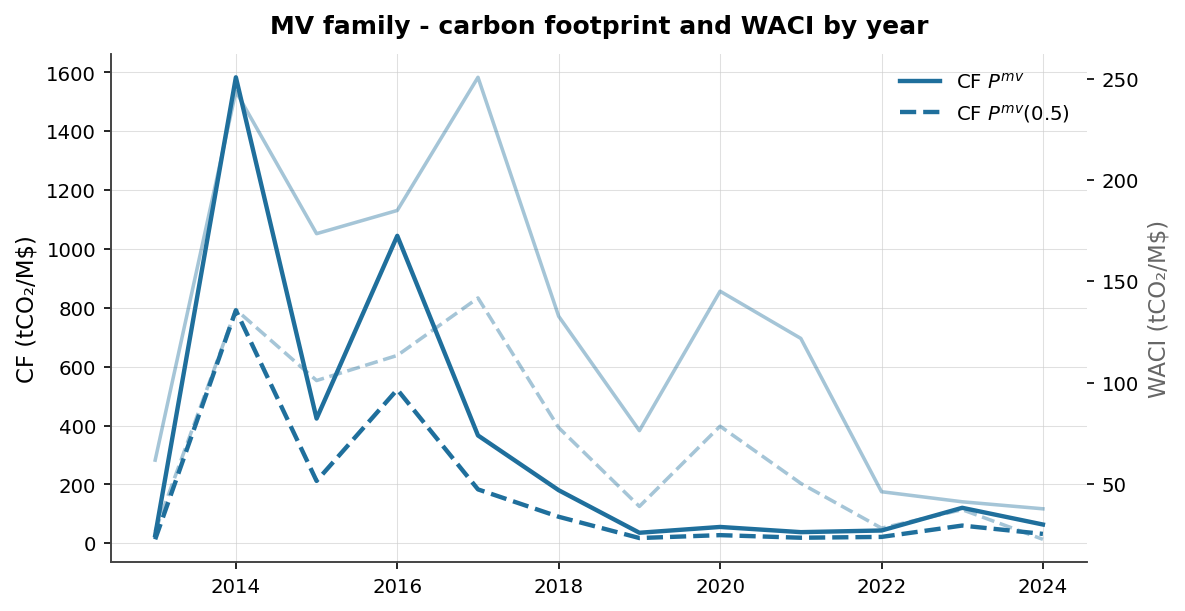
\includegraphics[width=0.78\linewidth]{part2_carbon_footprint_mv_family.png}
\caption{\textbf{Year-by-year carbon metrics of the minimum-variance
family, plotted on a stand-alone axis.} \emph{What:} WACI (left $y$
axis) and CF (right $y$ axis) of $P^{mv}$ and $P^{mv}(0.5)$ from
2013 to 2024. \emph{How constructed:} same formulas
(\ref{eq:waci})--(\ref{eq:cf}) as for the VW family, but plotted on
its own scale because the MV-family numbers are 5--10x smaller than
the VW family and become unreadable in the dual panel of
Figure~\ref{fig:part2-cf-split}. \emph{How to read:} both curves
are structurally low; the unconstrained $P^{mv}$ exhibits sharp
spikes in 2014--2017 driven by a single high-CI Russian steel name
(EVRAZ) that the variance optimiser briefly favours; the constrained
$P^{mv}(0.5)$ tames these spikes by construction because the cap is
recomputed every year as half of the unconstrained CF.}
\label{fig:mv-family-cf}
\end{figure}

Figure~\ref{fig:excess} translates the VW-family results into excess
returns vs.\ $P^{vw}$. The 50\%-cap portfolio drifts $\sim$5\%
below the benchmark over 12 years; the NZ portfolio drifts $\sim$4\%
below. Most of the cumulative drag accrues during 2020--2022, when
high-carbon energy and materials names rebounded strongly from the
2020 trough.

\begin{figure}[ht]
\centering
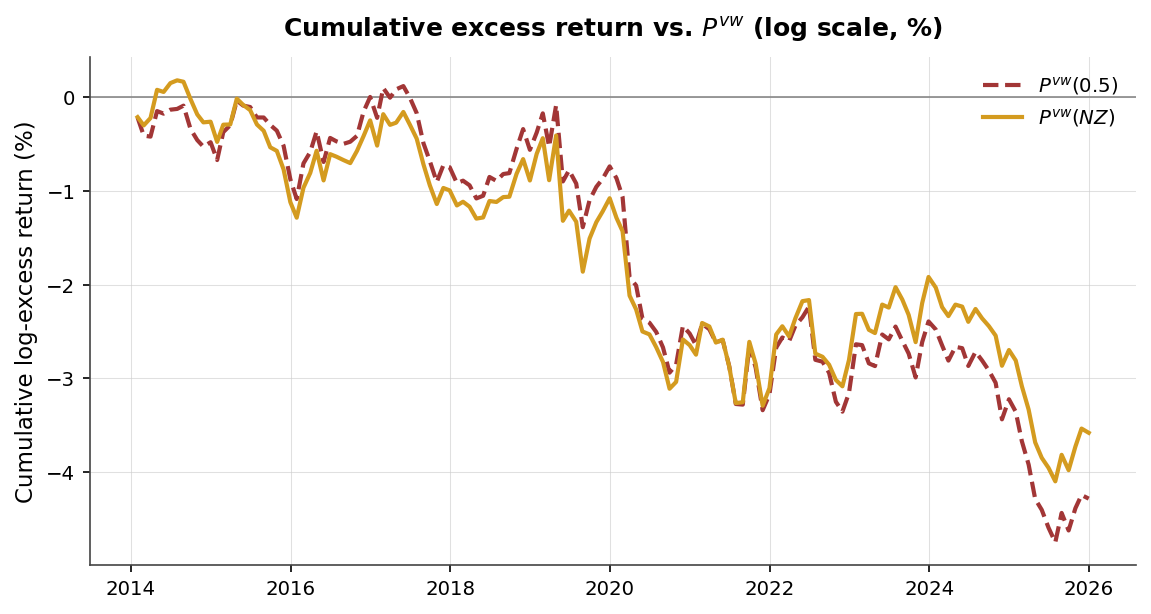
\includegraphics[width=0.78\linewidth]{part2_excess_return_vs_vw.png}
\caption{\textbf{Cumulative excess return of the carbon-constrained
VW portfolios relative to $P^{vw}$.} \emph{What:} cumulative
log-ratio $\ln(W^{p}_t / W^{vw}_t)$ for $p \in
\{P^{vw}(0.5), P^{vw}(NZ)\}$, Jan 2014 -- Dec 2025.
\emph{How constructed:} the OOS monthly returns of the constrained
portfolio and the benchmark are independently compounded and the
ratio is plotted on a logarithmic scale, so that a slope of $-1\%$
corresponds to $1\%$ of annualised under-performance.
\emph{How to read:} both constrained portfolios stay within $\pm 2\%$
of the benchmark until 2020, then drift $\sim$4--5\% below during
the 2020--2022 fossil-energy rebound, and partially recover in the
subsequent risk-off period. The 12-year cumulative drag (4--5\%
total, i.e.\ $\sim$$30$--$40$\,bp pa) is small in absolute terms
relative to the carbon savings achieved.}
\label{fig:excess}
\end{figure}

% =======================================================================
\section{Mathematical notes}\label{app:math}
% =======================================================================

\subsection{Squared vs.\ root tracking error}

The project specification states the tracking-error objective as
\(\text{TE}(P) = \sqrt{(w-w^{vw})'\Sigma(w-w^{vw})}\).
We implement the equivalent
\(\text{TE}^2(P) = (w-w^{vw})'\Sigma(w-w^{vw})\). Because the square-root
function is strictly increasing on $[0,\infty)$ and the squared TE is
non-negative on the feasible set, the two problems share the same
argmin:
\[
  \arg\min_{w\in\mathcal{F}} \sqrt{(w-w^{vw})'\Sigma(w-w^{vw})}
  \;=\;
  \arg\min_{w\in\mathcal{F}} (w-w^{vw})'\Sigma(w-w^{vw}).
\]
Working with the squared form avoids the non-differentiability of the
square root at zero and yields a closed-form quadratic objective that
SLSQP can exploit directly.

\subsection{KKT conditions for the carbon-constrained QP}

Problem~\eqref{eq:vw05} is a convex QP with feasible set
$\mathcal{F}=\{w:\mathbf{1}'w=1,\;0\le w\le \mathbf{1},\;c'w\le \bar c\}$,
where $c_i=E_{i,Y}/\text{MV}_{i,Y}$ and $\bar c=0.5\cdot CF(P^{vw})_Y$.
The KKT conditions at an optimum $w^*$ are
\begin{align*}
  2\,\Sigma(w^*-w^{vw}) - \lambda\,\mathbf{1} + \mu\,c + \nu_- - \nu_+ &= 0 \\
  \mathbf{1}'w^* &= 1 \\
  c'w^* &\le \bar c, \quad \mu\ge 0, \quad \mu\,(\bar c - c'w^*) = 0 \\
  0 \le w^*_i \le 1, \quad \nu_{-,i},\nu_{+,i}\ge 0 \\
  \nu_{-,i}\,w^*_i = 0, \quad \nu_{+,i}\,(1-w^*_i) = 0.
\end{align*}
In our runs, the cap is binding in every year ($\mu>0$ and
$c'w^*=\bar c$), and the bound constraints are typically active only on
high-carbon names that the optimiser zeros out --- i.e.\
$\nu_{-,i}>0,\;w^*_i=0$ for $i$ such that $c_i\gg \bar c$.

% =======================================================================
\section*{References}\addcontentsline{toc}{section}{References}
% =======================================================================

\begin{thebibliography}{9}
\bibitem[Andersson et al.(2016)]{AnderssonBoltonSamama2016}
  Andersson, M., Bolton, P., \& Samama, F. (2016).
  Hedging climate risk.
  \textit{Financial Analysts Journal}, \textbf{72}(3), 13--32.
\bibitem[Bolton \& Kacperczyk(2021)]{BoltonKacperczyk2021}
  Bolton, P., \& Kacperczyk, M. (2021).
  Do investors care about carbon risk?
  \textit{Journal of Financial Economics}, \textbf{142}(2), 517--549.
\bibitem[Clarke et al.(2006)]{Clarke2006MinVar}
  Clarke, R., De Silva, H., \& Thorley, S. (2006).
  Minimum-variance portfolios in the U.S. equity market.
  \textit{Journal of Portfolio Management}, \textbf{33}(1), 10--24.
\bibitem[Ledoit \& Wolf(2004)]{LedoitWolf2004}
  Ledoit, O., \& Wolf, M. (2004).
  Honey, I shrunk the sample covariance matrix.
  \textit{Journal of Portfolio Management}, \textbf{30}(4), 110--119.
\end{thebibliography}

\end{document}
